\chapter{Finitt Differanse Metode (FDM)}
FDM er en numerisk metode for å løse ODE og PDE ved å diskretisere domenet og tilnærme den deriverte med differanser.
\section{Motivasjon}
Gitt en vilkårlig differensiallikning (ODE), som f.eks. \( \ddn[2]{f(x)}{x} = f(x) - x^3 \)\label{eq:ode} med randbetingelser: \( f(x_0) = \alpha \) og \( f(x_N) = \beta \).
Denne ODE har allerede en eksakt løsning: \( f(x) = c_0e^x + c_1e^{-x} + x^3 + 6x \)\label{eq:exact}.
Men, hva om vi ikke har en eksakt løsning? Da kan vi bruke FDM til å tilnærme løsningen.

\section{FDM-oppskrift}
\begin{enumerate}
  \item \textbf{Diskretisering:} Del intervallet \(x \in [\alpha, \beta]\) inn i \(N\) like store delintervaller med \(x_i = \alpha + ih\) for \(i = 0,1,\ldots,N\) og \(h = 2/N\)
  \item \textbf{Taylor-utvikling:} Rekkeutvikle \(f(x \pm h)\) rundt \(x\).
  \item \textbf{Differanse metoder:} Finn en lineærkombinasjon av \(f(x \pm h)\) som tilnærmer den deriverte.
        \begin{align}
          C_{-1}f(x - h) + C_0f(x) + C_1f(x + h)   & = \ddn[f(x)]{2}{x} + \mathcolor{blue}{O(h)} \tag{Central} \label{eq:center}    \\
          C_{0}f(x) + C_1f(x + h ) + C_2f(x + 2h)  & = \ddn[f(x)]{2}{x} + \mathcolor{blue}{O(h^2)} \tag{Forward} \label{eq:forward} \\
          C_{-2}f(x - 2h) + C_{-1}f(x-h) + C_0f(x) & = \ddn[f(x)]{2}{x} + \mathcolor{blue}{O(h)} \tag{Backward} \label{eq:backward}
        \end{align}
  \item \textbf{Diskretiser og løs ODE:} Anvend en av disse metodene, f.eks. \ref{eq:center} på \ref{eq:ode} og løs ligningssettet \(T_h \vec{f} = \vec{b}\), hvor \(T_h\) er en tri-diagonal.
\end{enumerate}
\section*{Differanseoperatorer}

Differanseoperatorer er diskrete tilnærminger av deriverte og kan brukes til å konstruere differanseskjemaer for numerisk løsning av \gls{ode} og \gls{pde}.

\section{Grunnleggende differanseoperatorer}

Differanseoperatorer er fundamentale byggeklosser for diskretisering av deriverte, og danner grunnlaget for numeriske metoder for differensiallikninger.

\subsection{Fremover differanseoperator}
\begin{definition}{Fremover differanse}{}
  \begin{equation}
    \Delta_h u(x) = u(x + h) - u(x) \label{eq:forward_diff}
  \end{equation}
  der $h > 0$ er steglengden.
\end{definition}

\begin{remark*}{}{}
  Fremover differanse tilnærmer den første deriverte med nøyaktighet $O(h)$:
  \begin{equation}
    \frac{\Delta_h u(x)}{h} = u'(x) + \frac{h}{2}u''(x) + O(h^2)
  \end{equation}
\end{remark*}

\subsection{Bakover differanseoperator}
\begin{definition}{Bakover differanse}{}
  \begin{equation}
    \nabla_h u(x) = u(x) - u(x - h) \label{eq:backward_diff}
  \end{equation}
\end{definition}

\begin{remark*}{}{}
  Bakover differanse tilnærmer også den første deriverte med nøyaktighet $O(h)$, men bruker tidligere punkter:
  \begin{equation}
    \frac{\nabla_h u(x)}{h} = u'(x) - \frac{h}{2}u''(x) + O(h^2)
  \end{equation}
\end{remark*}

\subsection{Sentral differanseoperator}
\begin{definition}{Sentral differanse}{}
  \begin{equation}
    \delta_h u(x) = u(x + h/2) - u(x - h/2) \label{eq:central_diff}
  \end{equation}
\end{definition}

\begin{remark*}{}{}
  Sentral differanse gir en mer nøyaktig tilnærming av den første deriverte:
  \begin{equation}
    \frac{\delta_h u(x)}{h} = u'(x) + O(h^2)
  \end{equation}
  Dette gjør den til et foretrukket valg når høyere presisjon er nødvendig.
\end{remark*}

\subsection{Andre ordens sentral differanseoperator}
\begin{definition}{Andre ordens sentral differanse}{}
  \begin{equation}
    \delta_h^2 u(x) = u(x + h) - 2u(x) + u(x - h) \label{eq:second_central_diff}
  \end{equation}
\end{definition}

\begin{proposition}{Tilnærming til andre deriverte}{}
  Andre ordens sentral differanseoperator gir en approksimering av den andre deriverte med nøyaktighet $O(h^2)$:
  \begin{equation}
    \frac{\delta_h^2 u(x)}{h^2} = u''(x) + O(h^2)
  \end{equation}
\end{proposition}

\begin{remark*}{}{}
  Denne operatoren er spesielt nyttig for numerisk løsning av elliptiske og parabolske partielle differensiallikninger, som varmeledningslikningen og Poissons likning.
\end{remark*}

\subsection{Gjennomsnittsoperator}
\begin{definition}{Gjennomsnittsoperator}{}
  \begin{equation}
    \mu_h u(x) = \frac{1}{2} \left( u(x + h/2) + u(x - h/2) \right) \label{eq:avg_op}
  \end{equation}
\end{definition}

\begin{remark*}{}{}
  Gjennomsnittsoperatoren kan brukes til å konstruere differanseskjemaer med høyere nøyaktighet ved å kombinere fremover og bakover differanser.
  Den kan også brukes til å lage differanseskjemaer med høyere nøyaktighet ved å kombinere fremover og bakover differanser.
\end{remark*}

\subsection{Skiftoperator}
\begin{definition}{Skiftoperator}{}
  \begin{equation}
    E_h u(x) = u(x + h) \label{eq:shift_op}
  \end{equation}
\end{definition}

\begin{remark*}{}{}
  Skiftoperatoren kan brukes til å uttrykke alle andre differanseoperatorer, for eksempel:
  \begin{align}
    \Delta_h   & = E_h - I           \\
    \nabla_h   & = I - E_{-h}        \\
    \delta_h^2 & = E_h - 2I + E_{-h}
  \end{align}
  der $I$ er identitetsoperatoren, $Iu(x) = u(x)$.
\end{remark*}

\begin{theorem}{Differanseoperatorenes relasjoner}{}
  Differanseoperatorene er relatert til hverandre på følgende måter:
  \begin{align}
    \delta_h^2 & = \Delta_h \nabla_h = \nabla_h \Delta_h \\
    \delta_h   & = \mu_h \Delta_h = \mu_h \nabla_h E_h   \\
    E_h        & = I + \Delta_h
  \end{align}
  der $I$ er identitetsoperatoren, $Iu(x) = u(x)$.
\end{theorem}

\begin{remark*}{}{}
  Fremover- og bakover-differanseoperatorer er asymmetriske og gir første ordens nøyaktighet,
  mens sentral differanse er symmetrisk og gir andre ordens nøyaktighet ved tilnærming av første deriverte.
\end{remark*}

\begin{example}{Anvendelse av differanseoperatorer}{}
  For funksjonen $u(x) = x^2$ ved $x=1$ med $h=0.1$:
  \begin{align*}
    \Delta_h u(1)   & = (1+0.1)^2 - 1^2 = 1.21 - 1 = 0.21                       \\
    \nabla_h u(1)   & = 1^2 - (1-0.1)^2 = 1 - 0.81 = 0.19                       \\
    \delta_h^2 u(1) & = (1+0.1)^2 - 2(1^2) + (1-0.1)^2 = 1.21 - 2 + 0.81 = 0.02
  \end{align*}
  Dette stemmer overens med andre deriverte $u''(x) = 2$ siden $\frac{\delta_h^2 u(1)}{h^2} = \frac{0.02}{0.01} = 2$.
\end{example}

\begin{proposition}{Taylor-utvikling av differanseoperatorer}
  Differanseoperatorenes tilnærminger til deriverte kan uttrykkes ved Taylor-rekker:
  \begin{align*}
    \frac{\Delta_h u(x)}{h}     & = u'(x) + \frac{h}{2}u''(x) + O(h^2) \\
    \frac{\nabla_h u(x)}{h}     & = u'(x) - \frac{h}{2}u''(x) + O(h^2) \\
    \frac{\delta_h u(x)}{h}     & = u'(x) + O(h^2)                     \\
    \frac{\delta_h^2 u(x)}{h^2} & = u''(x) + O(h^2)
  \end{align*}
\end{proposition}

\subsection*{Stensiler}

\begin{figure}[H]
  \centering
  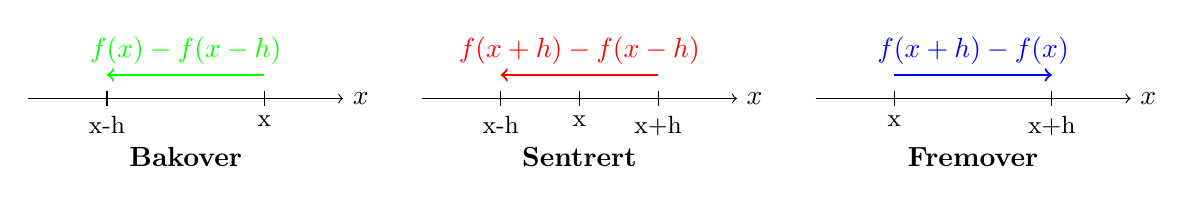
\begin{tikzpicture}
    % Backward Difference Scope
    \begin{scope}[xshift=-5cm]
      \draw[->] (-1,0) -- (3,0) node[right] {$x$}; % Number Line
      \foreach \x/\label in {0/$x-h$, 2/$x$} {
          \draw (\x,0.1) -- (\x,-0.1); % Points
          \node[below] at (\x,-0.1) {\small $\label$}; % Labels
        }
      \draw[->, thick, green] (2,0.3) -- (0,0.3) node[midway, above] {$f(x) - f(x-h)$}; % Arrow for difference
      \node[below] at (1, -0.5) {\textbf{Bakover}}; % Label
    \end{scope}

    % Central Difference Scope
    \begin{scope}[xshift=0cm]
      \draw[->] (-1,0) -- (3,0) node[right] {$x$};
      \foreach \x/\label in {0/$x-h$, 1/$x$, 2/$x+h$} {
          \draw (\x,0.1) -- (\x,-0.1); % Points
          \node[below] at (\x,-0.1) {\small $\label$};
        }
      \draw[->, thick, red] (2,0.3) -- (0,0.3) node[midway, above] {$f(x+h) - f(x-h)$};
      \node[below] at (1, -0.5) {\textbf{Sentrert}};
    \end{scope}

    % Forward Difference Scope
    \begin{scope}[xshift=5cm]
      \draw[->] (-1,0) -- (3,0) node[right] {$x$};
      \foreach \x/\label in {0/$x$, 2/$x+h$} {
          \draw (\x,0.1) -- (\x,-0.1);
          \node[below] at (\x,-0.1) {\small $\label$};
        }
      \draw[->, thick, blue] (0,0.3) -- (2,0.3) node[midway, above] {$f(x+h) - f(x)$};
      \node[below] at (1, -0.5) {\textbf{Fremover}};
    \end{scope}
  \end{tikzpicture}
  \caption{Finite Difference Stencils: Backward, Central, and Forward Difference}
  \label{fig:finite-differences}
\end{figure}


Som figuren viser, benytter \textbf{fremover}-differanser hovedsakelig punkter \emph{til høyre} for \(x_i\),
\textbf{bakover}-differanser benytter hovedsakelig punkter \emph{til venstre} for \(x_i\),
mens \textbf{sentrerte}-differanser er symmetriske rundt \(x_i\).


\section*{Endelig differanseskjema}

Endelige differanseformler gir diskrete tilnærminger av deriverte ved å bruke funksjonsverdier i strategisk utvalgte punkter (ofte kalt \emph{stencil}).
Kolonnene merket \(\mathbf{-3}\) til \(\mathbf{+3}\) (eller flere, avhengig av formelens bredde) oppgir \emph{dimensjonsløse koeffisienter} som multipliserer funksjonsverdiene i \(x_{i + k}\).

For å beregne den deriverte numerisk, må du så dividere med \(h^n\), der \(n\) er den deriverteordenen:

\[
  \frac{d^n f}{dx^n} \Bigg|_{x_i} \approx \frac{1}{h^n} \sum_{k=-m}^{m} \bigl( c_k f(x_{i+k}) \bigr)
\]

\begin{itemize}
  \item \(m\) er halvparten av stencilens bredde (f.eks. 3 for en 7-punkts stencil).
  \item \(c_k\) er dimensjonsløse koeffisienter.
\end{itemize}

\begin{table}[H]
  \centering
  \setlength{\tabcolsep}{5pt}
  \renewcommand{\arraystretch}{1.2}
  \begin{tabular}{|c|c|c|c|c|c|c|c|c|c|}
    \hline
    \rowcolor{cyan!20} \textbf{\footnotesize{Metode}} & \textbf{\footnotesize{Der.}} & \textbf{\footnotesize Acc.} & $\mathbf{-3}$    & $\mathbf{-2}$    & $\mathbf{-1}$   & $\mathbf{0}$     & $\mathbf{1}$      & $\mathbf{2}$       & $\mathbf{3}$     \\ \hline

    \multirow{12}{*}{\textbf{\footnotesize{Forover}}}
                                                      & \multirow{3}{*}{1}           & 2                           &                  &                  & $-1$            & $1$              &                   &                    &                  \\ \cline{3-10}
                                                      &                              & 4                           &                  & $\frac{1}{6}$    & $-\frac{2}{3}$  & $1$              &                   &                    &                  \\ \cline{3-10}
                                                      &                              & 6                           & $-\frac{1}{60}$  & $\frac{3}{20}$   & $-\frac{3}{4}$  & $1$              &                   &                    &                  \\ \cline{2-10}
                                                      & \multirow{3}{*}{2}           & 2                           &                  &                  & $1$             & $-2$             & $1$               &                    &                  \\ \cline{3-10}
                                                      &                              & 4                           &                  & $-\frac{1}{12}$  & $\frac{4}{3}$   & $-\frac{5}{2}$   & $\frac{4}{3}$     & $-\frac{1}{12}$    &                  \\ \cline{3-10}
                                                      &                              & 6                           & $\frac{1}{90}$   & $-\frac{3}{20}$  & $\frac{3}{2}$   & $-\frac{49}{18}$ & $\frac{3}{2}$     & $-\frac{3}{20}$    &                  \\ \cline{2-10}
                                                      & \multirow{3}{*}{3}           & 2                           &                  &                  & $-1$            & $3$              & $-3$              & $1$                &                  \\ \cline{3-10}
                                                      &                              & 4                           &                  & $\frac{1}{8}$    & $-1$            & $\frac{13}{8}$   & $-1$              & $\frac{1}{8}$      &                  \\ \cline{3-10}
                                                      &                              & 6                           & $-\frac{1}{120}$ & $\frac{1}{8}$    & $-1$            & $\frac{13}{8}$   & $-1$              & $\frac{1}{8}$      & $-\frac{1}{120}$ \\ \cline{2-10}
                                                      & \multirow{3}{*}{4}           & 2                           &                  &                  & $1$             & $-4$             & $6$               & $-4$               & $1$              \\ \cline{3-10}
                                                      &                              & 4                           &                  & $-\frac{1}{6}$   & $2$             & $-\frac{13}{2}$  & $\frac{28}{3}$    & $-\frac{13}{2}$    & $2$              \\ \cline{3-10}
                                                      &                              & 6                           & $\frac{1}{180}$  & $-\frac{2}{9}$   & $\frac{19}{18}$ & $-\frac{65}{18}$ & $\frac{916}{180}$ & $-\frac{65}{18}$   & $\frac{19}{18}$  \\ \hline

    \multirow{12}{*}{\textbf{\footnotesize{Sentrert}}}
                                                      & \multirow{3}{*}{1}           & 2                           &                  & $-\frac{1}{2}$   &                 & $\frac{1}{2}$    &                   &                    &                  \\ \cline{3-10}
                                                      &                              & 4                           & $\frac{1}{12}$   & $-\frac{2}{3}$   &                 & $\frac{2}{3}$    & $-\frac{1}{12}$   &                    &                  \\ \cline{3-10}
                                                      &                              & 6                           & $-\frac{1}{60}$  & $\frac{3}{20}$   & $-\frac{3}{4}$  &                  & $\frac{3}{4}$     & $-\frac{3}{20}$    & $\frac{1}{60}$   \\ \cline{2-10}
                                                      & \multirow{3}{*}{2}           & 2                           &                  & $\frac{1}{2}$    & $-1$            & $0$              & $1$               & $-\frac{1}{2}$     &                  \\ \cline{3-10}
                                                      &                              & 4                           &                  & $-\frac{1}{12}$  & $\frac{4}{3}$   & $-\frac{5}{2}$   & $\frac{4}{3}$     & $-\frac{1}{12}$    &                  \\ \cline{3-10}
                                                      &                              & 6                           & $-\frac{1}{90}$  & $\frac{3}{20}$   & $-\frac{3}{2}$  & $\frac{49}{18}$  & $-\frac{3}{2}$    & $\frac{3}{20}$     & $\frac{1}{90}$   \\ \cline{2-10}
                                                      & \multirow{3}{*}{3}           & 2                           &                  & $-\frac{1}{2}$   & $1$             & $0$              & $-1$              & $\frac{1}{2}$      &                  \\ \cline{3-10}
                                                      &                              & 4                           &                  & $\frac{1}{8}$    & $-1$            & $\frac{13}{8}$   & $-1$              & $\frac{1}{8}$      &                  \\ \cline{3-10}
                                                      &                              & 6                           & $\frac{1}{90}$   & $-\frac{3}{20}$  & $\frac{3}{2}$   & $-\frac{13}{8}$  & $1$               & $\frac{3}{20}$     & $-\frac{1}{90}$  \\ \cline{2-10}
                                                      & \multirow{3}{*}{4}           & 2                           &                  & $1$              & $-4$            & $6$              & $-4$              & $1$                &                  \\ \cline{3-10}
                                                      &                              & 4                           &                  & $-\frac{1}{6}$   & $2$             & $-\frac{13}{2}$  & $\frac{28}{3}$    & $-\frac{13}{2}$    & $2$              \\ \cline{3-10}
                                                      &                              & 6                           & $\frac{1}{180}$  & $-\frac{2}{9}$   & $\frac{19}{18}$ & $-\frac{65}{18}$ & $\frac{916}{180}$ & $-\frac{65}{18}$   & $\frac{19}{18}$  \\ \hline

    \multirow{12}{*}{\textbf{\footnotesize{Bakover}}}
                                                      & \multirow{3}{*}{1}           & 2                           &                  & $1$              & $-1$            &                  &                   &                    &                  \\ \cline{3-10}
                                                      &                              & 4                           &                  & $-\frac{1}{6}$   & $\frac{2}{3}$   & $-1$             &                   &                    &                  \\ \cline{3-10}
                                                      &                              & 6                           & $\frac{1}{60}$   & $-\frac{3}{20}$  & $\frac{3}{4}$   & $-1$             &                   &                    &                  \\ \cline{2-10}
                                                      & \multirow{3}{*}{2}           & 2                           &                  & $-1$             & $2$             & $-1$             &                   &                    &                  \\ \cline{3-10}
                                                      &                              & 4                           &                  & $\frac{1}{12}$   & $-\frac{4}{3}$  & $\frac{5}{2}$    & $-\frac{4}{3}$    & $\frac{1}{12}$     &                  \\ \cline{3-10}
                                                      &                              & 6                           & $-\frac{1}{90}$  & $\frac{3}{20}$   & $-\frac{3}{2}$  & $\frac{49}{18}$  & $-\frac{3}{2}$    & $\frac{3}{20}$     & $-\frac{1}{90}$  \\ \cline{2-10}
                                                      & \multirow{3}{*}{3}           & 2                           &                  & $1$              & $-3$            & $3$              & $-1$              &                    &                  \\ \cline{3-10}
                                                      &                              & 4                           &                  & $-\frac{1}{8}$   & $1$             & $-\frac{13}{8}$  & $1$               & $\frac{1}{8}$      &                  \\ \cline{3-10}
                                                      &                              & 6                           & $\frac{1}{90}$   & $-\frac{3}{20}$  & $\frac{3}{2}$   & $-\frac{13}{8}$  & $1$               & $\frac{3}{20}$     & $-\frac{1}{90}$  \\ \cline{2-10}
                                                      & \multirow{3}{*}{4}           & 2                           &                  & $-1$             & $4$             & $-6$             & $4$               & $-1$               &                  \\ \cline{3-10}
                                                      &                              & 4                           &                  & $\frac{1}{6}$    & $-2$            & $\frac{13}{2}$   & $-\frac{28}{3}$   & $\frac{13}{2}$     & $-2$             \\ \cline{3-10}
                                                      &                              & 6                           &                  & $-\frac{1}{180}$ & $\frac{2}{9}$   & $-\frac{19}{18}$ & $\frac{65}{18}$   & $-\frac{916}{180}$ & $\frac{65}{18}$  \\ \hline
  \end{tabular}
  \caption{Koeffisienter for endelige differanser for deriverte opptil fjerde orden.
    Kolonnene \(\mathbf{-3}\) til \(\mathbf{+3}\) (eller mer) viser de dimensjonsløse koeffisientene i front av \(f(x_{i+k})\).
    Til slutt divideres sumproduktet med \(h^n\) for en \(n\)-te deriverte.
    «Acc.» angir den formelle nøyaktighetsordenen.}
  \label{tab:finite_difference_table}
\end{table}

\vspace{1em}

\noindent\textbf{Tips for bruk:}
\begin{itemize}
  \item Kontroller alltid \emph{tegnkonvensjon og indeksering} \(\;f(x_{i+k}) \leftrightarrow \text{koeffisient under kolonne }k\).
  \item Etter at koeffisientene er multiplisert med funksjonsverdiene, \emph{deler med} \(h^n\) for en \(n\)-te deriverte.
  \item Fremover/bakover brukes ofte nær kantene av et domene for å unngå ute-av-rekkevidde-punkter.
  \item Sentrerte differanser gir vanligvis høyere nøyaktighet enn fremover- eller bakoverdifferanser, siden de utnytter symmetrien rundt punktet ved å bruke naboverdier likt på begge sider.
\end{itemize}




\subsubsection{Bakover differanseoperator}
\begin{align*}
  \nabla_h u_m & = u_m - u_{m-1}                                                                                                                            \\
               & = u_m - \left[u_m - h u_m^{\prime} + \frac{h^2}{2} u_m^{\prime\prime} - \frac{h^3}{6} u_m^{(3)} + \frac{h^4}{24} u_m^{(4)} - \hdots\right] \\
               & = h u_m^{\prime} - \frac{h^2}{2} u_m^{\prime\prime} + \frac{h^3}{6} u_m^{(3)} - \frac{h^4}{24} u_m^{(4)} + \hdots                          \\
               & = h u_m^{\prime} + O(h^2)                                                                                                                  \\
               & = O(h)
\end{align*}

\begin{align*}
  \nabla_h^2 u_m & = u_m - 2u_{m-1} + u_{m-2}                                                                                                                   \\
                 & = u_m                                                                                                                                        \\
  - 2            & \left[u_m - h u_m^{\prime} + \frac{h^2}{2} u_m^{\prime\prime} - \frac{h^3}{6} u_m^{(3)} + \frac{h^4}{24} u_m^{(4)} - \hdots\right]           \\
  +              & \left[u_m - 2h u_m^{\prime} + \frac{4h^2}{2} u_m^{\prime\prime} - \frac{8h^3}{6} u_m^{(3)} + \frac{16h^4}{24} u_m^{(4)} - \hdots\right]      \\
                 & = h^2 u_m^{\prime\prime} - 2h^2 u_m^{\prime\prime} + \frac{2h^3}{3} u_m^{(3)} - \frac{4h^3}{3} u_m^{(3)} + \frac{4h^4}{3} u_m^{(4)} - \hdots \\
                 & = h^2 u_m^{\prime\prime} - h^3 u_m^{(3)} + \frac{7h^4}{12} u_m^{(4)} + O(h^5)                                                                \\
                 & = h^2 u_m^{\prime\prime} - h^3 u_m^{(3)} + O(h^4)                                                                                            \\
                 & = O(h^2)
\end{align*}

\begin{align*}
  \nabla_h^3 u_m & = u_m - 3u_{m-1} + 3u_{m-2} - u_{m-3}                                                                                                    \\
                 & = u_m                                                                                                                                    \\
  - 3            & \left[u_m - h u_m^{\prime} + \frac{h^2}{2} u_m^{\prime\prime} - \frac{h^3}{6} u_m^{(3)} + \frac{h^4}{24} u_m^{(4)} - \hdots\right]       \\
  + 3            & \left[u_m - 2h u_m^{\prime} + \frac{4h^2}{2} u_m^{\prime\prime} - \frac{8h^3}{6} u_m^{(3)} + \frac{16h^4}{24} u_m^{(4)} - \hdots\right]  \\
  -              & \left[u_m - 3h u_m^{\prime} + \frac{9h^2}{2} u_m^{\prime\prime} - \frac{27h^3}{6} u_m^{(3)} + \frac{81h^4}{24} u_m^{(4)} - \hdots\right] \\
                 & = h^3 u_m^{(3)} - 3h^3 u_m^{(3)} + \frac{3h^4}{2} u_m^{(4)} - \frac{9h^4}{2} u_m^{(4)} + \hdots                                          \\
                 & = h^3 u_m^{(3)} - \frac{3h^4}{2} u_m^{(4)} + O(h^5)                                                                                      \\
                 & = h^3 u_m^{(3)} + O(h^4)                                                                                                                 \\
                 & = O(h^3)
\end{align*}

\begin{example}{}{}
  \( f''(x) = f(x) - x^3 \) med \( [f(0), f(2)] = [0, 20] \) og \( N = 5 \). Det gir 1D FDM-ligningssettet med sentral differanseoperator:
  \begin{align*}
    \overbrace{
      \begin{bmatrix}
        1             & 0                  & 0             & \cdots & 0             \\
        \frac{1}{h^2} & -\frac{2}{h^2} - 1 & \frac{1}{h^2} & \cdots & 0             \\
        0             & \ddots             & \ddots        & \ddots & \vdots        \\
        \vdots        & \ddots             & \ddots        & \ddots & \frac{1}{h^2} \\
        0             & \cdots             & 0             & 0      & 1
      \end{bmatrix}}^{L_h}
    \overbrace{
      \begin{bmatrix}
        f(x_0) \\ f(x_1) \\ \vdots \\ f(x_{N-1}) \\ f(x_N)
      \end{bmatrix}}^{\vec{f}}
                & =
    \overbrace{
    \begin{bmatrix}
        \alpha \\ h^2(x_1^3 - x_1) \\ \vdots \\ h^2(x_{N-1}^3 - x_{N-1}) \\ \beta
      \end{bmatrix}}^{\vec{b}} \\
    L_h \vec{f} & = \vec{b}\tag{SUS!}
  \end{align*}

  \vspace{0.5em}

  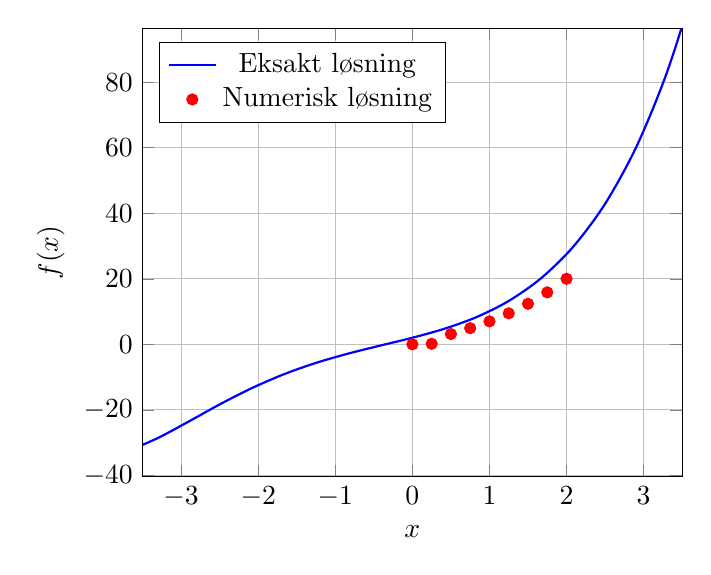
\begin{tikzpicture}
    \begin{axis}[
        xlabel={\(x\)},
        ylabel={\(f(x)\)},
        grid=major,
        legend pos=north west,
        xmin=-3.5,
        xmax=3.5,
        xtick={-3, -2, -1, 0, 1, 2, 3},
      ]
      \addplot[smooth, thick, blue] {x^3 + 6*x + exp(x) + exp(-x)};
      \addplot[only marks, red] coordinates {
          (0, 0)
          (0.25, 0.1516)
          (0.5, 3.125)
          (0.75, 4.922)
          (1, 7)
          (1.25, 9.453)
          (1.5, 12.375)
          (1.75, 15.859)
          (2, 20)
        };
      \legend{Eksakt løsning, Numerisk løsning}
    \end{axis}
  \end{tikzpicture}
  \label{fig:ode}
\end{example}

